\section{Modélisation des données}
Commentaire : la modélisation des données est la modélisation statique en UML.  Elle contient aussi le MCD et le schéma de la base de données.

\subsection{Diagramme de classe (UML)}
Commentaire.  Indiquez les classes de données utilisées dans l’application.  Toutes les données utilisées dans l’application doivent s’y trouver.

\subsection{Modèle conceptuel de données (MCD)}
Commentaire.  Utilisez un modèle entité-relation pour décrire l’organisation des données de l’application.  Vérifiez que le modèle respecte TOUTES les formes normales.

\begin{center}
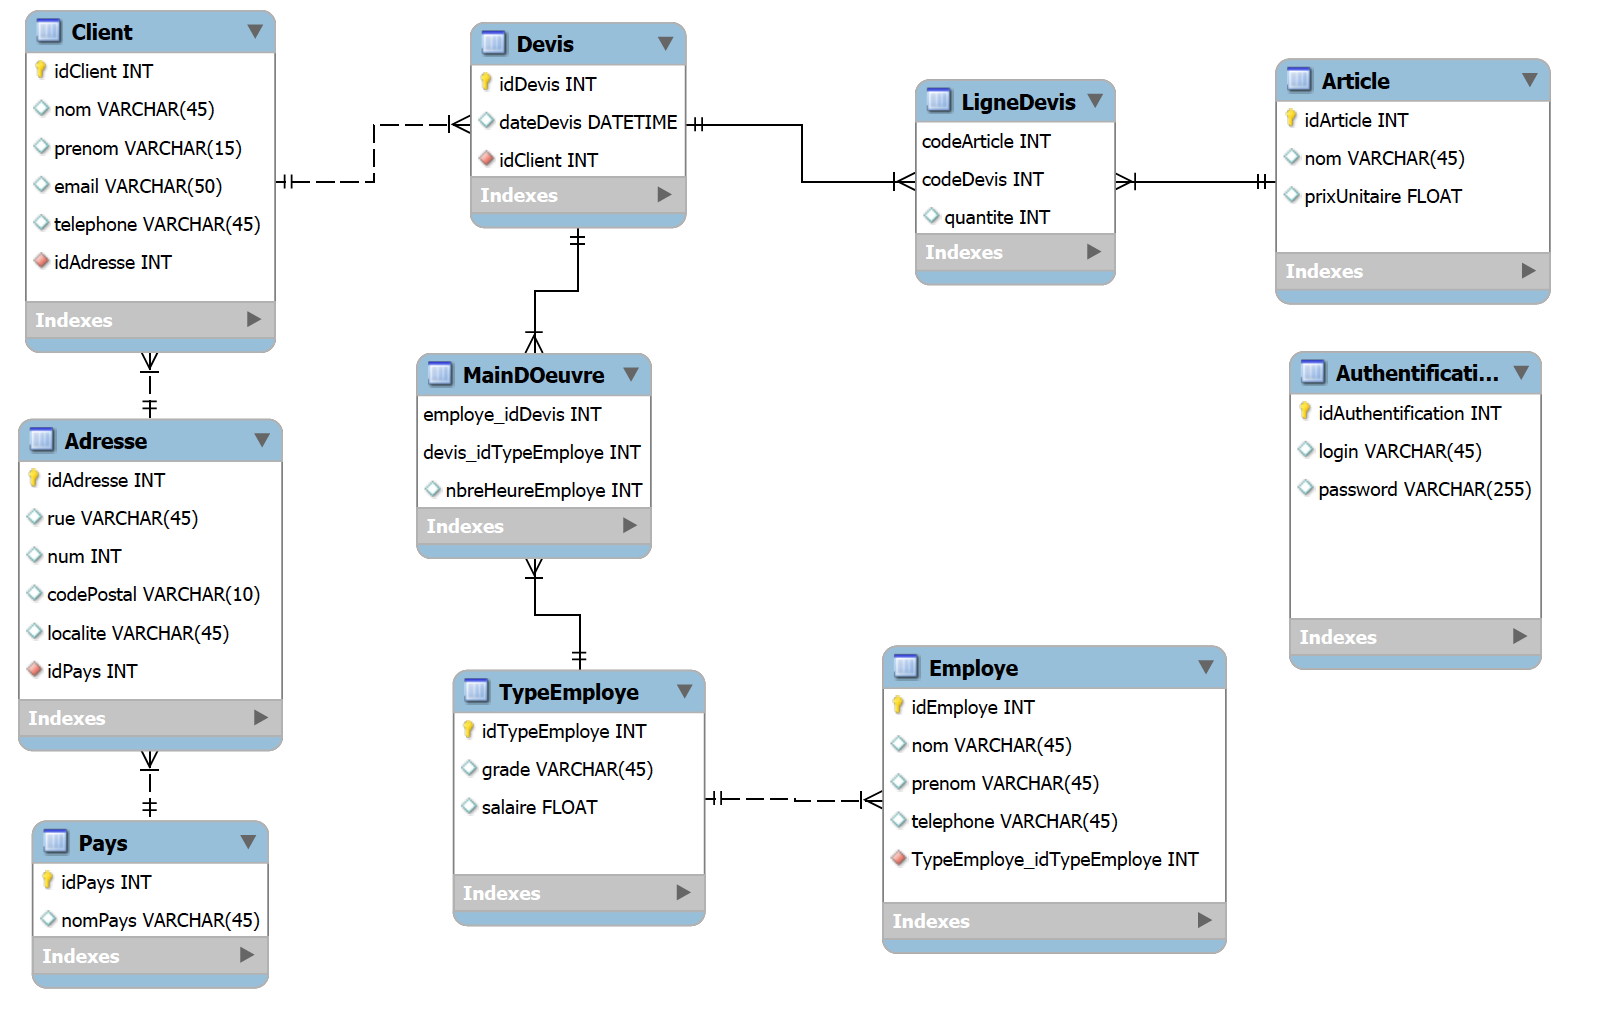
\includegraphics[scale=0.5]{images/projetDevis.png}
\end{center}

\subsection{Modèle de la base de données}
Commentaire.  La modélisation de la base de données représente comment sont organisées les données quand elles sont stockées.  Elle décrit le schéma de la base de données.

\subsection{Documentation des données}
Commentaire.  Toutes les données utilisées dans l’application doivent être documentées dans le tableau ci-dessous.
